\documentclass[12pt]{article}
\usepackage{ITTol-Reporte}	

% Paquete usado para incluir texto falso (Lorem Ipsum) en el ejemplo 
% Opciones pangram, bible, random (defecto)
\usepackage[pangram]{blindtext}
\usepackage{lipsum}	
\usepackage{apacite}		

%%%%%%%%%%%%%%%%%%%% MODIFICAR %%%%%%%%%%%%%%%%%%%%%%
\title{Instituto Tecnológico de Toluca}
\author{
  Autor1 Nombre Apellidos  \inst{1}, 
  Autor2 Nombre Apellidos  \inst{2}, 
  Autor3 Nombre Apellidos   \inst{1}
}
\address{
  División de Estudios de Posgrado e Investigación (DEPI) -- 
  Instituto Tecnológico de Toluca (ITTol)\\
  Metepec; Estado de México México
\nextinstitute
  Departamento de Ciencias Computacionales\\
  Universidad del estado de México (UAEMex) 
  Toluca; Estado de México México
  \email{
     autor1@toluca.tecnm.mx, 
     autor2@uaemex.mx,
     autor3@toluca.tecnm.mx}
}
%%%%%%%%%%%%%%%%%%%% OBLIGATORIOS %%%%%%%%%%%%%%%%%%%%
\newcommand{\IT}{Instituto Tecnológico de Toluca}
\newcommand{\proyecto}{Nombre del Proyecto}
\newcommand{\fecha}{Octubre de 2022}
%%%%%%%%%%%%%%%%%%%%%%%%%%%%%%%%%%%%%%%%%%%%%%%%%

%%%%%%%%%%%%%%%%%%%% NÃO ALTERAR %%%%%%%%%%%%%%%%
%%%%%configurando referências de acordo com a ABNT
%%%%\usepackage[alf]{abntex2cite}
%%%%%\usepackage{fancyhdr}
%%%%\fancyhead{} % clear all header fields
%%%%\renewcommand{\headrulewidth}{0pt} % no line in header area
%%%%\fancyfoot{} % clear all footer fields
%%%%\fancyfoot[R]{ \vspace{2pt} \footnotesize \thepage}           % page number in "outer" position of footer line
%%%%%\fancyfoot[RE,LO]{Instituto Federal de Pernambuco. \textit{Campus} \campus. Curso de \curso. \dataaprovacao. } % 
%%

%%%%%%%%%%%%%%%%%%%% NO MODIFICAR %%%%%%%%%%%%%%%%%%%%
\fancyhead{}   									% clear all header fields
\renewcommand{\headrulewidth}{0pt} 				% no line in header area
\fancyfoot{} 									% clear all footer fields
\fancyfoot[R]{ \vspace{2pt} \footnotesize \thepage}             % page number in "outer" position of footer line
\fancypagestyle{firststyle}
{
   \fancyfoot[L]{TecNM / \IT. \\
    \proyecto. / \fecha.} % 
}
\pagestyle{firststyle}
\sloppy


%%%%%%%%%%%%%%%%%%%%%%%%%%%%%%%%%%
% Documento
%%%%%%%%%%%%%%%%%%%%%%%%%%%%%%%%%%
\begin{document} 

%%%%%%%%%%%%%%%%%%%%%%%%%%%%%%%%%%%
%% Institución, Proyecto, Autores, Direcciones
\maketitle
\thispagestyle{firststyle}
\hrule

%%%%%%%%%%%%%%%%%%%%%%%%%%%%%%%%%%%
%% Resumen - Abstract
\begin{resumen} 			% Resumen en español
  \lipsum[1]	    		         % Reemplazar por el texto del resumen
 
  \textbf{Palabras clave:} Red Neuronal, Inteligencia Artificial, ...
\end{resumen}

\selectlanguage{english}            % Resumen en inglés
\begin{abstract}				 % Reemplazar por el texto del resumen en inglés
  \lipsum[1]
  
  \textbf{Keywords:}  Neural network, Artificial Intelligence
\end{abstract}
\selectlanguage{spanish}
\hrule

%%%%%%%%%%%%%%%%%%%%%%%%%%%%%%%%%%%
% Introducción
\section{Introducción}

\lipsum[1-2] 
Como se puede apreciar en la Figura \ref{fig:01_Proceso}.

\begin{figure}[htbp]                                                      % Inclusión de una figura
\centering
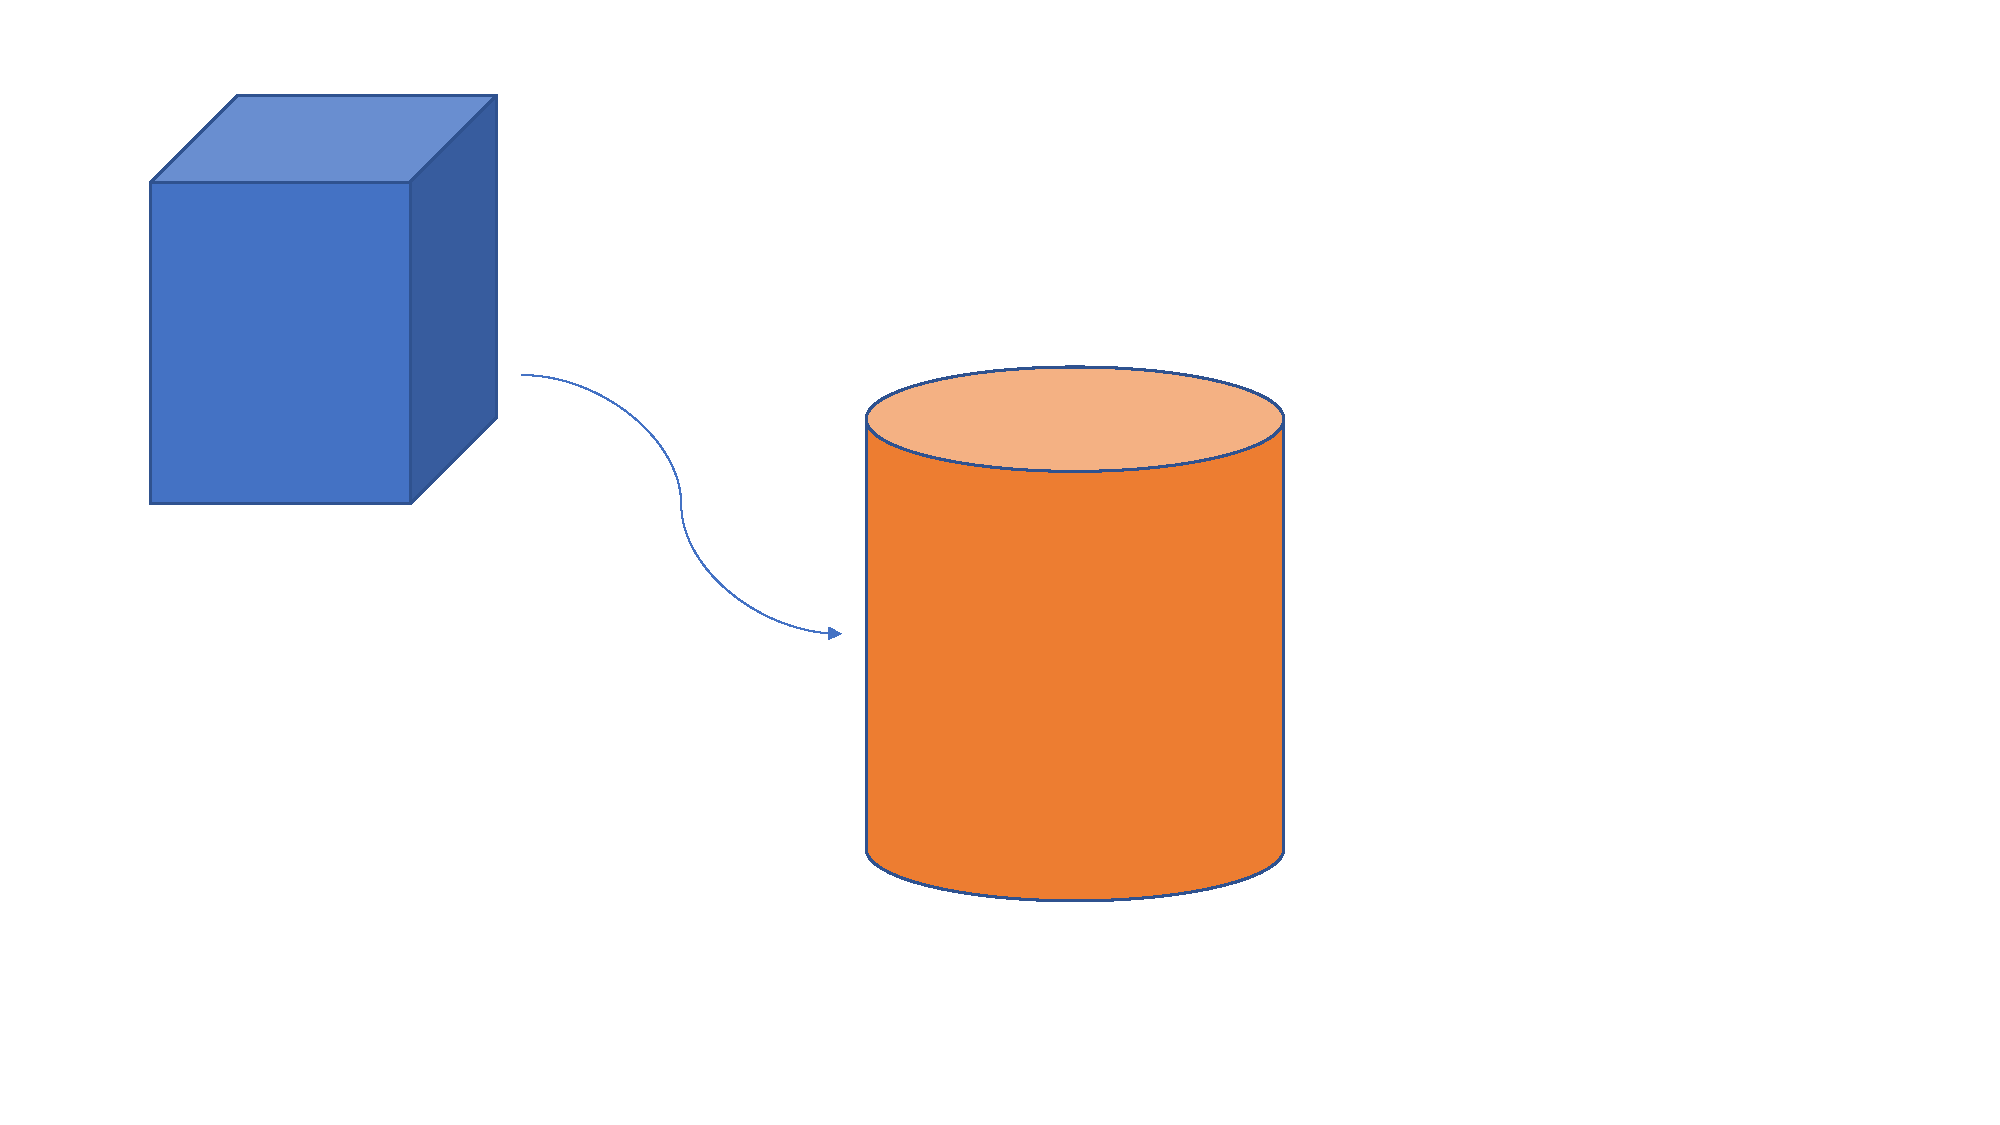
\includegraphics[width=0.80\textwidth]{a_Imagen01}
\caption{Donec vehicula augue eu neque.}
\label{fig:01_Proceso}
\end{figure}

\subsection{Ejemplo Link}
\lipsum[1]
En el \href{https://es.wikipedia.org/wiki/Proceso_(ingenier%C3%ADa)}{Wikipedia - Proceso} se pueden consultar la descripción
del proceso mostrado en la Figura~\ref{fig:01_Proceso}. 


%%%%%%%%%%%%%%%%%%%%%%%%%%%%%%%%%%%
% Fundamentos
\section{Fundamentos Teóricos}
\lipsum[1].

\begin{equation}                                                     
\mathrm{e}^{x} = \sum_{k=0}^{\infty} \frac{x^k}{k!} = 
1 + x + \frac{x^2}{2} + \frac{x^3}{6} + \cdots
\label{eq:taylor}
\end{equation}

La ecuación \eqref{eq:taylor} muestra la expansión en serie de Taylor alrededor de $x = 0$ para la función exponencial natural.


%%%%%%%%%%%%%%%%%%%%%%%%%%%%%%%%%%%
% Metodología
\section{Metodología}
\lipsum[1-2]. 
Se recomienda atender las recomendaciones y buena prácticas indicadas en su seminario de investigación, de tesis, o de
las referencias bibliográficas pertinentes, por ejemplo \cite{Sampieri}

\section{Ejemplo Algoritmo}
\lipsum[1]

El análisis de datos se realiza con el Algoritmo \ref{Alg:Algo-01}, descrito en seguida:

\begin{algorithm}[H]
  \SetAlgoLined
  \KwData{this text}
  \KwResult{how to write algorithm with \LaTeX2e }
  initialization\;
  \While{not at end of this document}{
    read current\;
    \eIf{understand}{
      go to next section\;
      current section becomes this one\;
      }{
      go back to the beginning of current section\;
      }
    }
  \caption{How to write algorithms}
  \label{Alg:Algo-01}
\end{algorithm}


%%%%%%%%%%%%%%%%%%%%%%%%%%%%%%%%%%%
% Resultados
\lipsum[1].  
Los resultados pueden verse en la Tabla \ref{tab:Tabla1}

\begin{table}[htbp]
\centering
\caption{Resultados obtenidos.}
\label{tab:pversust}
\begin{tabular}{>{\itshape}l<{:} *{2}{l}}
  \toprule
  Animal  & Comida & Tamaño  \\
  \midrule
  perro   & carne  & mediano \\
  caballo & heno   & grande  \\
  rana    & moscas & pequeño \\
  \bottomrule
\end{tabular}
\label{tab:Tabla1}
\end{table}

\lipsum[2]

\section{Ejemplo Figura}
\lipsum[3-4]

\begin{figure}[!tbp]
\centering
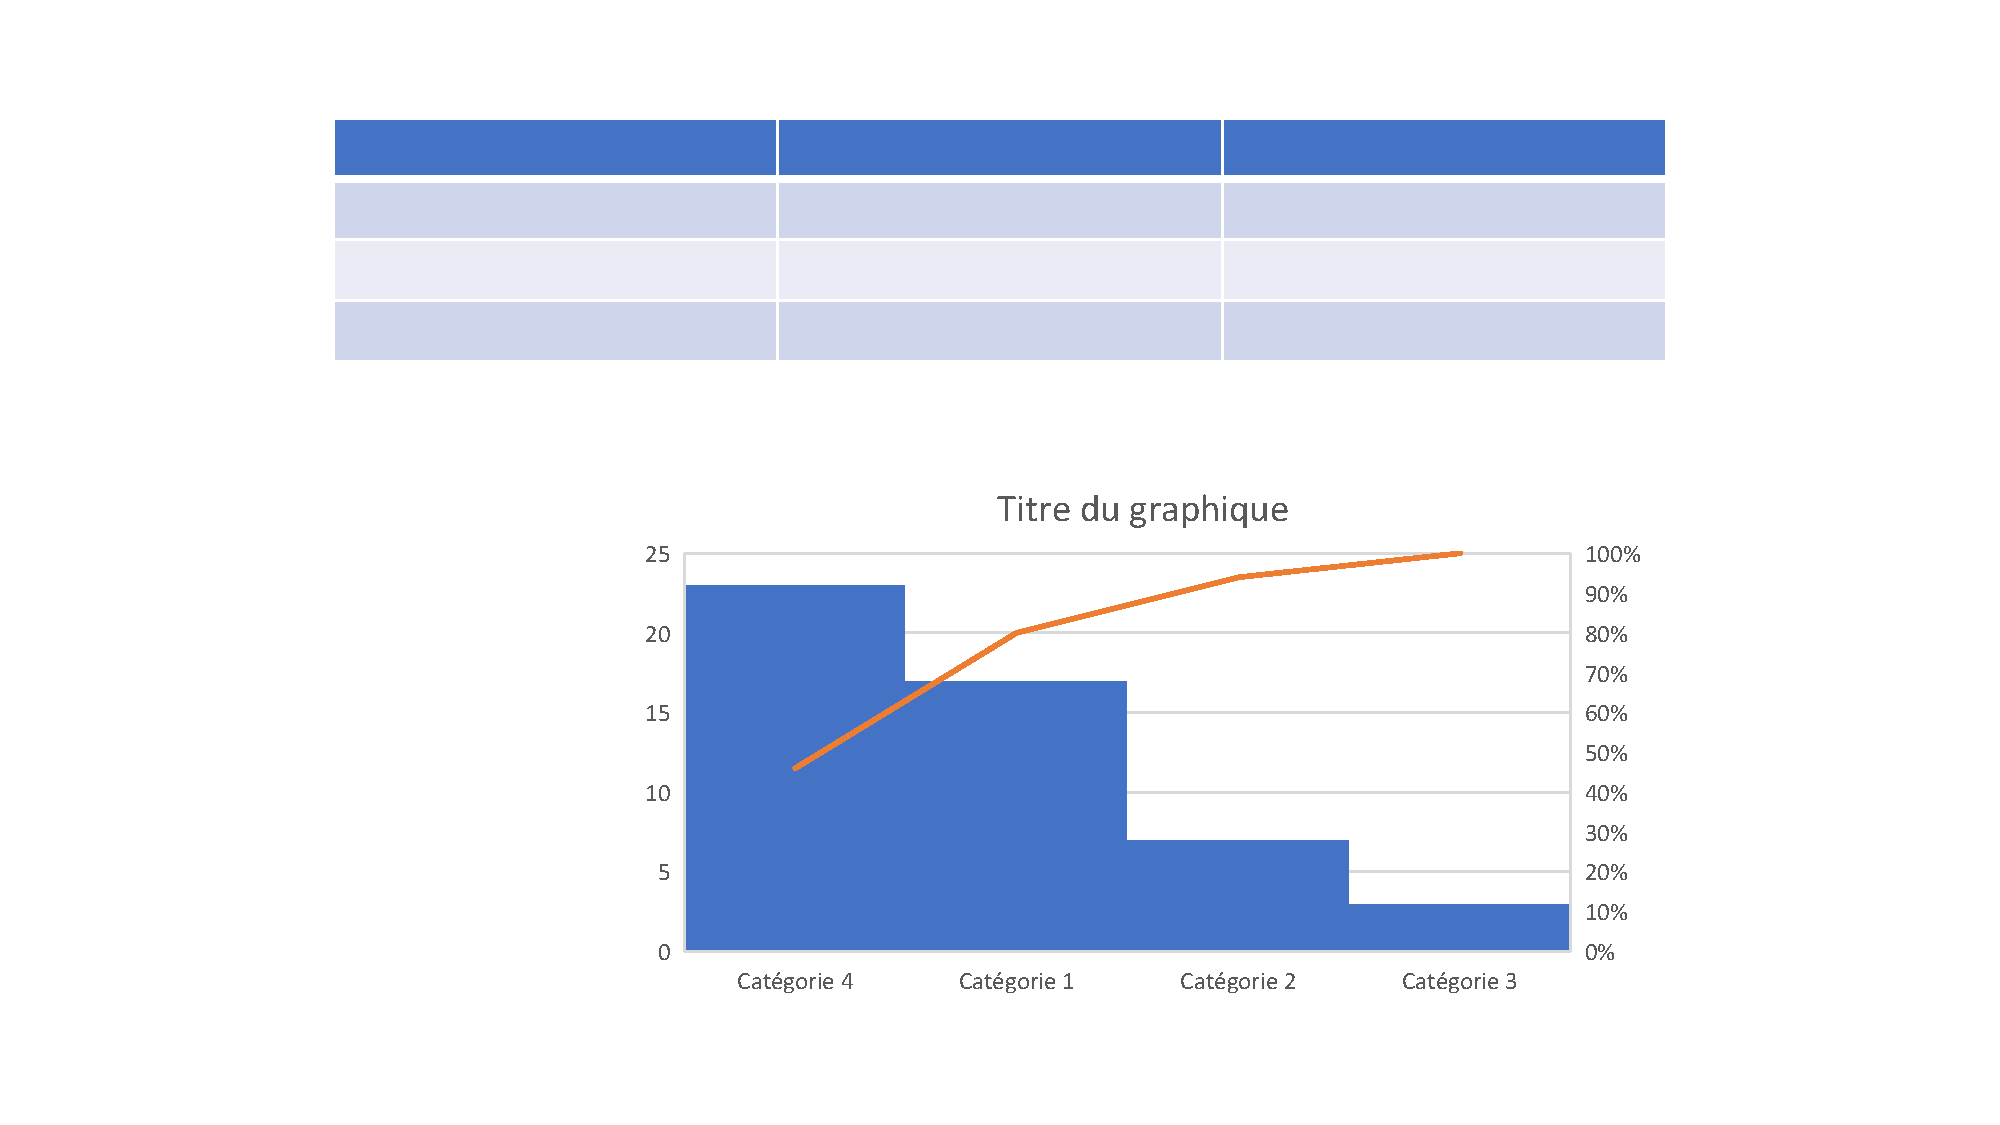
\includegraphics[width=0.50\textwidth]{e_Imagen01}
\caption{Duis eget orci sit amet orci dignissim rutrum.}
\label{fig:particion}
\end{figure}


%%%%%%%%%%%%%%%%%%%%%%%%%%%%%%%%%%%
% Código fuente
\section{Código fuente}
\lipsum[1-2]
\noindent
Escribe el siguiente programa en un archivo llamado \texttt{hola.c}:

\begin{lstlisting}[style=C]
#include <stdio.h>

int main(int argc, char* argv[]) 
{
    printf("Hola mundo!");
}
\end{lstlisting}

\noindent
Ahora compila usando \texttt{gcc}:

\begin{listing}[style=terminal, numbers=none]
$ gcc  -o hola hola.c
\end{listing}


% Bibliografía
%%%%%%%%%%%%%%%%%%%%%%%%%%%%%%%%%%
\bibliographystyle{apacite}
\bibliography{biblio}								% Archivo .bib
\nocite{*}

\end{document}

